\documentclass[dvipdfmx]{standalone} % $B=q<0(Bstandalone$B$G(Bdvipdfmx$B$r;H$C$F(BPDF$B@8@.(B
%\documentclass[dvipdfmx]{jsarticle} % $B=q<0(Bstandalone$B$G(Bdvipdfmx$B$r;H$C$F(BPDF$B@8@.(B
\usepackage{tikz} % tikz$B%Q%C%1!<%8$rFI$_9~$`(B
\usetikzlibrary{shadows}

%%%
%%%
\definecolor{cyan10}{cmyk}{.1,0,0,0}
\definecolor{cyan20}{cmyk}{.2,0,0,0}
\definecolor{cyan30}{cmyk}{.3,0,0,0}
\definecolor{cyan40}{cmyk}{.4,0,0,0}
\definecolor{cyan50}{cmyk}{.5,0,0,0}
\definecolor{cyan60}{cmyk}{.6,0,0,0}
\definecolor{cyan70}{cmyk}{.7,0,0,0}
\definecolor{cyan80}{cmyk}{.8,0,0,0}
\definecolor{cyan90}{cmyk}{.9,0,0,0}
\definecolor{or1}{cmyk}{.05,.19,.89,0}
\definecolor{or2}{cmyk}{0,.58,.91,0}


\begin{document} % document$B4D6-3+;O(B

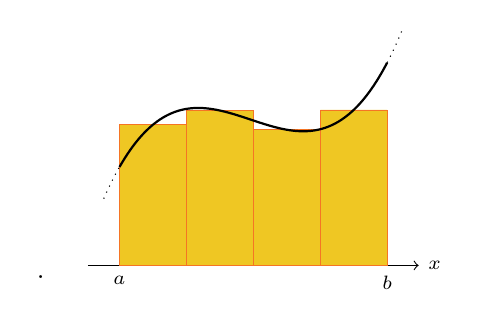
\begin{tikzpicture}[domain=-2:2, samples=100, thick,scale=2] % $BDj5A0h!"E@$N?t!"@~I}(B
%\draw (0,0) node[below left]{O}; 
\draw[thin, ->] (-0.7,0)--(1.4,0) node[right] {{\scriptsize $x$}}; 
%\draw[thin, ->] (0,-0.5)--(0,3.5) node[above] {{\scriptstyle $y$}}; % y$B<4(B
%%
%\draw[thin,dashed](-1,0)--(-1,0);  
%\filldraw[thin,draw=cyan80,
 %fill=cyan20](-1,2)--(1,2)--(1,0)--(-1,0)--(-1,2);
\filldraw[very thin,draw=or2, fill=or1](-0.500000,0.893580)--(-0.075000,0.893580)--(-0.075000,0.0)--(-0.500000,0.0)--(-0.500000,0.893580);
\filldraw[very thin,draw=or2, fill=or1](-0.075000,0.983693)--(0.350000,0.983693)--(0.350000,0.0)--(-0.075000,0.0)--(-0.075000,0.983693);
\filldraw[very thin,draw=or2, fill=or1](0.350000,0.861572)--(0.775000,0.861572)--(0.775000,0.0)--(0.350000,0.0)--(0.350000,0.861572);
\filldraw[very thin,draw=or2, fill=or1](0.775000,0.987811)--(1.200000,0.987811)--(1.200000,0.0)--(0.775000,0.0)--(0.775000,0.987811);
%\draw (0,0) node[below]{{\scriptstyle $c$}};  
%%
\draw[thick,domain=-0.5:1.2] plot(\x, \x*\x*\x-\x*\x+1); 
\draw[thin,dotted,domain=-0.6:-0.5] plot(\x, \x*\x*\x-\x*\x+1); 
\draw[thin,dotted,domain=1.2:1.3] plot(\x, \x*\x*\x-\x*\x+1); 
%\draw[thin,dotted,domain=1:1.3] plot(\x, {exp(0.6*\x)-\x*\x+1}); 
%\draw[thin,dotted,domain=-1.3:-1] plot(\x, {exp(0.6*\x)-\x*\x+1});
%%
\draw (-0.5,0) node[below]{{\scriptsize $a$}};
\draw (1.2,0) node[below]{{\scriptsize $b$}};
\draw (-1,0) node[below]{{.}};
\end{tikzpicture}

\end{document} % document$B4D6-=*N;